
\chapter{Ryanodine and Ryanodine Receptor}
\label{chap:ryan-ryan-recept}

The primary intracellular $\Ca$ storage in most cells is the sarcoplasmic
reticulum (SR) (in striated muscles (skeletal + cardiac)) or endoplasmic
reticulum (ER) (in non-muscle cell types). $\Ca$ are released from ER/SR via
specialized $\Ca$ release channels, with Ryanodine Receptor (RyR) for SR, and
Inositol-1,4,5-triphosphate receptors (IP$_3$R) for ER, each with three
different isoforms.
Chapter~\ref{chap:ip3r-models} discussed IP$_3$R. In this chapter, we will focus
on RyR.

\section{Ryanodine}
\label{sec:ryanodine}

Ryanodine - a plant alkaloid - is a poisonous alkaloid found in a plant named
Ryania speciosa (Flacourtiaceae). 

Ryanodine has high affinity to Ryanodine Receptors (Sect.\ref{sec:ryr}).
At nM level, ryanodine locks RyRs at sub-conductance state (i.e. channel
opening); while at micromolar level ($\mu$M), ryanodine completely close the
RyRs. So, it's dangerous when having nM level of ryanodine in body, as it cause
``leaky'' $\Ca$ from these excitable cells, causing massive muscular
contractions.



\section{RyR}
\label{sec:ryr}
\label{sec:introduction_ryr}
\label{sec:RyR}

Ryanodine receptor refers to the receptor that has high affinity to Ryanodine
(Sect.\ref{sec:ryanodine}). Ryanodine was found to bind to this protein in late
1980s, allowing purification and molecular charactarization of this protein.
Since then, ryanodine-receptor (RyR) was given to the name of the protein. RyR
is the only target of ryanodine reported today (2011).

RyR is an intracellular $\Ca$-gating proteins found in skeletal cell and heart
muscle cells, as well as in brain. Ryanodine receptors (RyRs) are found on
sarcoplasmic reticulum (SR) of striated muscles and serve as gates to release
\ce{Ca^2+} during the process known as \hyperref[sec:cicr]{CICR}
(\ce{Ca^2+}-induced \ce{Ca^2+}-released). There are totally 3 forms of RyRs have
been identified: RyR1, RyR2, RyR3\citep{rosemblit1999icr}.

\begin{itemize}
\item RyR1 expressed predominantly in skeletal muscle (in adult)

\item \textcolor{red}{RyR2 expressed dominantly in cardiac muscles} (in adult)

\item RyR3 expressed in specialized muscles and non-muscle tissues
  including the brain
\end{itemize}



Ultrastructure studies shown that, depending on species, there are a few tens to
200 RyR2s clustered into a 2D crystal-lattice array on the surface of SR release
terminals, apposed, across the 15-nm cleft of the diad junction, to the cluster
of DHPRs.

\begin{mdframed}
  RyR2 is a homotetramer of a polypeptide of roughly 5000 amino
  acids. The transmembrane \ce{Ca^2+}-sensitive domain is the
  COOH-terminal $\tilde{}$ 600 amino acids; the remainder of the
  molecule forms a 30-nm quatrefoil ``foot process'' that spans the
  dyadic cleft, and is required for the interaction of the channel
  with a variety of modulators.
\end{mdframed}

Recent data shows the evidence of structural-function
relationship~\citep{ikemoto2002rcr}. The N-terminal and the central
domain form a pair whose unzipping and zipping determines the opening
and closing probability of RyR, respectively.
\begin{itemize}
\item Unzipping lead to RyR2 hyperactivation (i.e. increase open
  prob.) and increase \ce{Ca^2+} leak from SR, ultimately causing
  heart failure.

\item Mutations in the three domains of RyR2 were reported to cause
  defective in inter-domain interaction; thus cause abnormal
  \ce{Ca^2+} cycling or leading to severe heart failure and lethal
  arrhythmia~\citep{tateishi2009ddd}.
\end{itemize}




\subsection{Sequences and Isoforms}
\label{sec:RyR_sequence_isoforms}


RyR is a complex protein (a tetramer), composed of 4 identical subunits and 4
KF506-binding proteins \citep{Coronado1994}. Each subunit is approximately 4810 amino
acids with molecular mass of about 560 kDa, and molecular mass of each FK506-binding
protein is 12 kDa. 

There are three known isoforms of RyR with the expression of different RyR
protein isoforms is tissue specific.
\begin{enumerate}
  \item RyR1 found in skeletal muscle~\citep{Takeshima1989,Zorzato1990}

  \item RyR2 found in cardiac cells~\citep{Nakai1990,Otsu1990}

  \item RyR3 found in brain~\citep{Hakamata1992}
\end{enumerate}
In fish, there may be a fourth type of RyR, i.e.
RyR-slow~\citep{Morrissette2000}.

RyR1 and RyR2 are $\tilde{}\;\; 66\%$ identical at amino acid level, as
shown in Fig.~\ref{fig:RyR_topo}~\citep{marks1997icr}. RyR3 is most
homologous to RyR2.

\begin{itemize}
\item In skeletal muscle: Four FKBP12 (aka FK506 binding protein 1A,
  12kDa) bind to each RyR complex (RyR1) (1 for each subunit in the
  channel)

\item In cardiac muscle: Four FKBP12.6 (aka FK506 binding protein 1B,
  12.6kDa) bind to each RyR complex (RyR2)
\end{itemize}
KFBP12 (as well as KFBP12.6) enhances the cooperation among the 4 RyR
subunits, resulting to more channel open to full conductance state
(i.e. all four pores in a ``large'' channel open) and close tightly,
thus preventing a leak of \ce{Ca^2+} from the SR.

\begin{figure}[hbt]
  \centerline{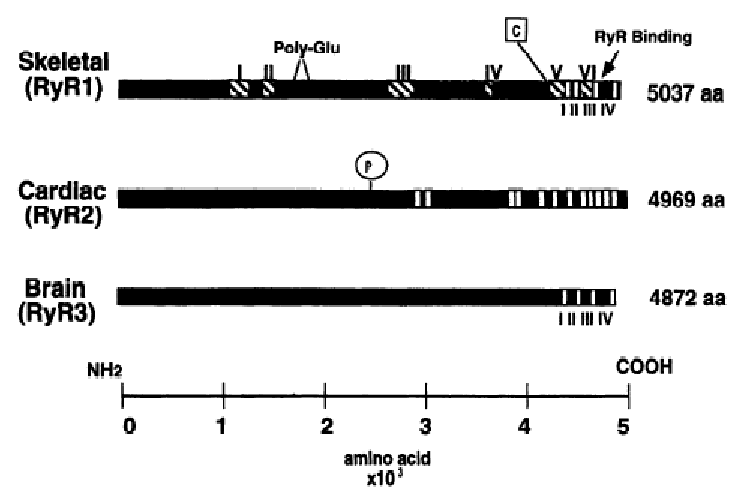
\includegraphics[height=6cm]{./images/RyR_topography.eps}}
  \caption{Proposed topography of RyR (1,2, and 3). A Polyglutamic
    region (Poly-Glu) is unique to RyR1.}
  \label{fig:RyR_topo}
\end{figure}

\begin{framed}
  At the amino-acid level, the 3 isoforms of RyR share $\sim 70\%$
  identity [....]. The analysis of the RyR 's primary amino acid
  sequence reveals many consensus ligand binding (ATP, $\ca$,
  caffeine, and CaM) and phosphorylation sites.

  \begin{itemize}

    \item E3882A (substitution alanine-3882 by glutamate) in RyR3 alters
    $\ca$ sensitivity. This imply this region contains the ``$\ca$
    sensor'' of the channel.
  
    \item hydrophobic FKBP12.6 binding sites comprised of isoleucine
    2427 and proline 2428, homologous to FKBP12 binding site in RyR1,
    IP3R1 and T$\beta$RI.
  
    \item ...
  \end{itemize}
\end{framed}

In humans, the  three genes (RyR1, RyR2, RyR3) are located in chromosome 19, 1,
and 15, respectively. There are also alternative splicing variants of RyR1 and
RyR2, but there functionality remains to be studied \citep{sutko1996}.

In terms of sequence similarity:
\begin{itemize}
  
  \item RyR2 human is 97\% closed to RyR2 mouse, 67\%
closed to RyR3 rabbit, and very low to other isoforms of RyRs from other species
  
  \item RyR1 human is 96\% closed to RyR1 pig/rabbit, 74\% closed to RyR1 fish,
64\% closed to RyR2 mouse and 65\% closed to RyR2 human.
\end{itemize}
The reason for low similarity of RyR isoforms is that there is a divergence in
the three domains: D1 (amino acid from 4254-4631), D2 (a.a. from 1342-1403) and
D3 (a.a. 1872-1923). D2 is completely absent in RyR3. 


%\subsection{Primary structure}
%\label{sec:primary-structure}

RyR2 macromolecule is a homotetramer with roughly 5,000 amino
acids. Each subunit is 565,000 dalton (i.e. 565kDa) RyR2 polypeptides,
containing a C-terminal (transmembrane domain) and N-terminal
(cytoplasmic domain). The idea of C-terminal is sufficient to form a
functional $\ca$ release channel was tested on skeletal cell of
Chinese hamster ovary (CHO)~\citep{Bhat1997}, and the N-terminal
affect the ion-conduction and $\ca$-dependent regulation of the $\ca$
release channel. 

\begin{framed}

  \textcolor{red}{RyR macromolecular complexes include FKBP12.6
  (Sect.\ref{sec:FKBP}), PKA (Sect.\ref{sec:PKA}), PKA regulatory subunit (RII)
  - Sect.\ref{sec:PKA-RyR}), the phosphatase PP1, PP2A, and an muscla A kinase
  anchoring protein mAKAP}\footnote{mAkAP
    binds PKA and targets to its substrates, PP1 and PP2A are major phosphatase
    proteins in cardiac muscles~\citep{MacDougall1991}}.
\end{framed}


\begin{figure}[hbt]
  % \centerline{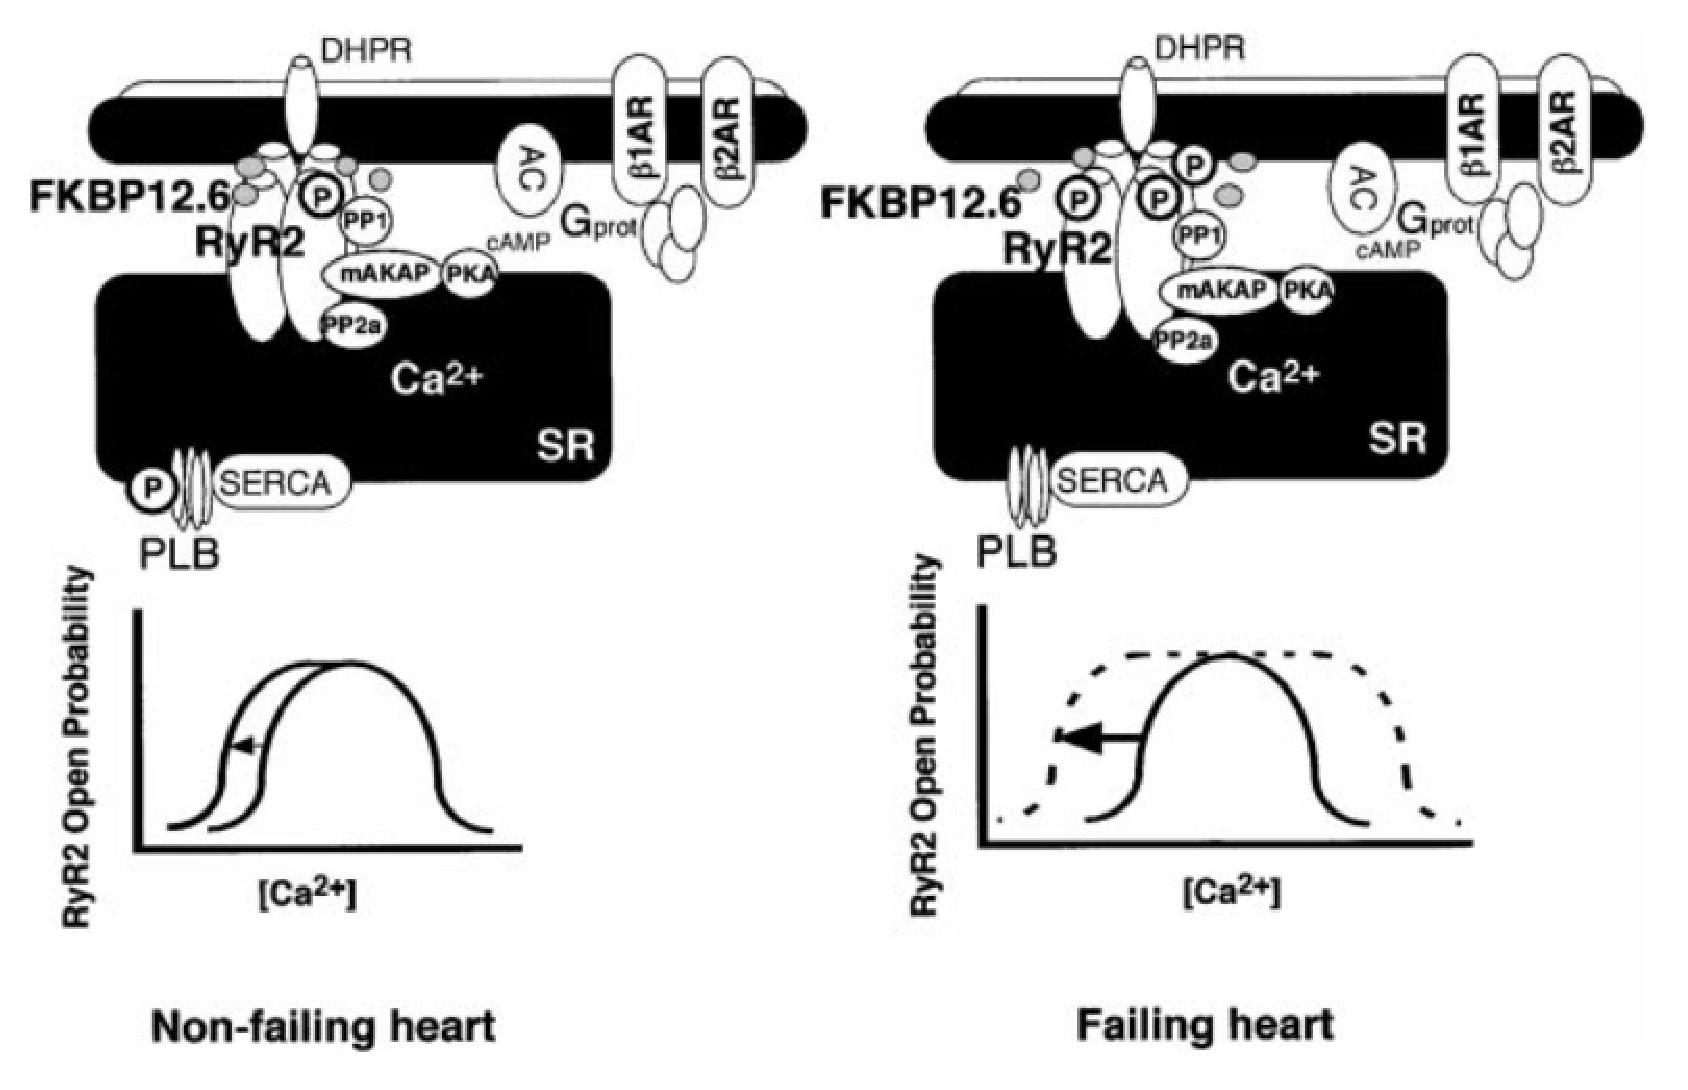
\includegraphics[height=5cm,
  %   angle=0]{./images/PKA_phosphorylation_RyR.eps}}
  \caption{$\beta$-agonists bind to receptors ($\beta 1$AR, $\beta
    2$AR) coupled to heterotrimeric G-protein (Gprot), which in turn
    activate adenylyl cyclase (AC), raising cAMP level and activating
    PKA. (Right) RyR2 channels in failing heart exhibit a shift in
    $\ca$-dependence activation, e.g. activate at resting level of
    cytosolic $\ca$~\citep{marx2000}}
  \label{fig:PKA_phosphorylation}
\end{figure}


\subsection{Non-mammalian RyR}

On non-mammalian vertebrates (birds, amphibians, reptiles and fish), RyRs are
known as $\alpha$-type, $\beta$-type and cardiac type. In amphibian (e.g.
bullfrog), $\alpha$-RyR and $\beta$-RyR isoforms are similar to RyR1 and RyR3
mammalian isoforms, respectively \citep{ogawa1994, ottini1996}. 

%   In non-mammalian cells, the RyR nomenclature is somewhat
%   difference, i.e. they contains nearly equal amount of 2 different
%   RyR proteins $\alpha$-RyR and $\beta$-RyR. They are homologs of
%   mammalian RyR1 and RyR3 respectively.
%   Example: RyR3 in rabbit brain is the homologue of bullfrog $\beta$-RyR. 


\subsection{3D structure}
\label{sec:RyR_3D}

RyR structures were first detected, though with a low resolution 30$\AA$, using
image processing techniques applied to electron micrograph of frozen-hydrated
purified channels. The landmark was RyR1~\citep{Radermacher1994},
RyR2~\citep{Sharma1998}, RyR3~\citep{Jeyakumar1998a}). Three isoforms resemble a
mushroom with a ``cap'' (or foot-like structre (foot-process) as seen under
electron micrographs of skeletal muscles) composed of the cytoplasmic domain and
the ``stalk'' made-up of the transmembrane (TM) domains
\citep{franzini_armstrong1994}.
Structures of higher resolution have been achieved, at
14$\AA$~\citep{Serysheva2004,Serysheva2005}, and 9.6$\AA$ using single-particle
electron microscopy of frozen purified channels
(cryo-EM)~\citep{Ludtke2005,samso2005}.

A truncated version of RyR with only the 276 residues of N-terminal and 1484
residues of C-terminal (carboxyl-terminal) can also function properly. This
suggests that the $\Ca$ conduction pore locates at the RyR C-terminus
\citep{Bhat1997, xu2000}. Using hydropathy plots, there are 2 suggested topology
models for this C-terminus: 4TM~\citep{Takeshima1989} and
10TM~\citep{Zorzato1990, orlova1996, sharma2000}.
The four segments of 4TM model correspond to M5, M6, M8 and M9 of the 10TM
model, in which it's suggested that M5-M9 forms part of the ion conduction
port (P-loop) and thus should not be considered as membrane spanning
\citep{balshaw1999}. \textcolor{red}{Nowadays, 10TM model is the favoured one.}

\begin{framed}
To detect if a domain is transmembrane, hydrophobicity of each amino-acid can be
calculated, and plotted. The resulting {\bf hydropathy plot} is used to predict
membrane spanning domain. To be a membrane spanning domain, there must be 20-25
very hydrophobic aminoa acids. If  this occurs, there is a good likelihood that
the sequence is transmembrane (TM) domain.
\end{framed}

For the pore structure, the critical sequence that involve in cation
transportation and selection is a conserved GGIG motif (residues 4894-4898 in
RyR1 within domain M9), a sequence related to GGI(V)G motif in IP3R and VGYG
motif in the unrelated class voltage-gated $\K$ channel that comprise the ion
selectivity filter \citep{doyle1998}.

Mutations in this motif, and neighboring residues create profound alterations in
RyR channel activity (i.e. cation conductance, and selectivity). Mutation G4824A
in RyR2 (equivalent to G4894A in RyR1) between M3 and M4 alters channel
conductance (reduce 97\% from 798 pS (picosiemens) WT to 22 pS) without
affecting channel activity. Co-expression of both WT and mutated proteins
produce individual channels of intermediate conductance: 516, 256, 176, and 60
pS \citep{zhao1999}. 

The same effect with mutation in the M10 helix, suggesting it forms the inner
helix of the pore.
\textcolor{blue}{Mutations at M9 and M10 are often found in skeletal and cardiac
muscle disease}. To maintain the high rate of cation transportation, a presence
of rings of negative charges in the luminal (D4899, E4900) and cytosolic (D4938
and D4945) vestibules is requierd.

Regulatory proteins are: Calmodulin (CaM), FKBP12.6, protein phosphatase I and
II (to be discussed further in Sect.\ref{sec:ryr_regulation-factors}). The
binding sites for two accessory proteins: calmodulin (CaM) and FKBP12 (or
FKBP12.6 in RyR2) are located further than 10nm from the putative TM pore. This
suggests that conformational change can be transmitted for a long distance.

\subsection{distribution}
 
\subsection{-- skeletal muscle}
\label{sec:RyR1}

RyR1 is coupled to a ``voltage-sensor''in the plasma membrane. Thus, the
activation of RyR1 is known as depolarization-induced calcium release (DICR)
mechanism which is found dominantly in striated muscles[...pg895].

RyR1 function is also regulated by
\begin{enumerate}
  
  \item  the transient receptor potential channel canonical type 3 (TRPC3) -
  Sect.\ref{sec:TRPC}
  
  \item  
\end{enumerate}



\subsection{-- cardiac muscle}
\label{sec:RyR2}

RyR2 is found dominantly in cardiac muscle.

\subsection{-- brain}

In neurons, IP3R is an important $\Ca$ release channels (Sect.\ref{sec:IP3R}).
However, evidences of IP3-insensitive yet caffeine-sensitive $\Ca$ release
channels have also found in neurons.
(Thayer et al., 1988a, 1988b) showed that ryanodine can block caffeine-induced
$\Ca$ release in sensory and sympathetic neurons
(Sect.\ref{sec:sensory_neuron}).

(McPherson and Campbell, 1990) showed that RyRs present in membranes from
throughout the brain and is enriched in membranes from the hippocampus .
When reconstituted into planar lipid bilayers, the brain ryanodine receptor
forms a caffeine- and ryanodine-sensitive Ca2+ channel with a 107 pS slope
conductance \citep{McPherson1991}.

An antibody raised against the synthetic peptide corresponding to amino acid
sequence 4375-4387 of rabbit RyR3 also interact with bullfrog $\beta$-RyR.
However, this antibody is not interacting with RyR1-2; and thus can be used to
identify the presence of RyR3 in rabbit brain.

Sucrose gradient ultracentrifugation revealed that RyR3 forms a homotetramer, as
true of the other isoforms. Being consistent with the distribution of its RNA,
RyR3 was abundantly expressed in {\bf hippocampus}, {\bf corpus striatum}, and
diencephalon (Sect.\ref{sec:diencephalon}).

Based on its dominant distribution on a given cell type, RyR1 is known as
skeletal type, RyR2 is cardiac type. RyR3 was also initially, though misleading,
called brain type.  In deed, RyR3 has a wide distribution among cell types; and
its level in brain is very low (with RyR2 is the major brain isoform), i.e.
the highest level found in mammals found at diaphragm muscle is still lower than
5\%~\citep{Murayama1997}. In another study on rabbit brain, [3H]Ryanodine
binding gave an estimate of RyR3 which would be only 2\% or less of total RyR in
rabbit brain \citep{Murayama1996}.

. A comprehensive review can be read
in~\citep{Zissimopoulos2007}. 

RyR3 is found mainly in mammalian striated muscles, but at a relatively low
level[...].


Physiological roles of RyRs were studied using gene knock-out method, at which
RyR1/2-deficient mouses show a decrease in skeletal and muscle contraction
function, i.e. altered EC-coupling. In contrast, there is no significant change
with RyR3-deficient cells, except during the first few weeks after birth. This
suggests a role of RyR3 in neonatal stage of muscle cells. Other
physiological roles of RyR3 were also found to affect learning
capabilities~\citep{Futatsugi1999}.

% \subsection{Permeability}
% \label{sec:permeability}




\subsection{Binding sites}

It is assumed multiple-ion binding sites are arranged sequentially, with $\Ca$
binding is favoured over monocation binding \citep{zucchi1997}. It's also
suggested a four-barrier, 3 binding-site model \citep{Tinker1992}.

\subsection{Mutations and diseases}

Until 2006, there are 70 mutations found in RyR2 that shown link to at least two
types of sudden cardiac death (SCD) \citep{thomas2006}: CPVT and ARVD2
(arrhythmogenic right ventricular cardiomyopathy type 2). Both are
autosomal dominantly inherited disorders.
\begin{enumerate}
  \item CPVT is characterized by adrenergic (or exercise)-induced ventricular
  tachycardia (with no structural disorder)
  \item ARVD2 is characterized by progressive degeneration of the right
  ventricular myocardium and arrhythmias. 
\end{enumerate} 

\subsection{Localization}
\label{sec:RyR_localization}

To detect RyR,  RyR antibodies labeled with Atto 647N can be used (ATTO 647N=a
new generation of fluorescent labels for the red spectral region, highly
suitable for single molecule detection using high-resolution microscopy like
STED, PALM, dSTORM, etc.).

RyR resides at the terminal cisternae (TC) of the SR (aka the junctional SR) at
which the junction between SR and plasma membrane is formed
(Sect.\ref{sec:junction-ER-plasmamembrane}).
In skeletal muscle cells, TC can face either the surface membrane to form
``peripheral coupling'' or the T-tubules to yield the ``triads''
(Sect.\ref{sec:triad}). In cardiac muscle, instead of a triad, it forms
``diad''. The reason is that number of TC is quantatively less numerous than
that in skeletal muscle cells.

Every four DHPR in skeletal muscle (DHPR$_s$) form a tetrad in which each
channel is linked to a subunit of the underlying RyR1.
However, DHPR in cardiac cell (DHPR$_c$) are randomly distributed w.r.t.
RyR2 array. There is no evidence for direct physical interaction between
DHPR$_c$ and RyR2. However, DHPR$_c$-RyR2 are coupled together under the
$\Ca$-induced $\Ca$-released mechanism \citep{fabiato1979cir}. It has been
estimated that the opening of a single DHPR$_c$ can atrigger $\Ca$ release from
4-6 RyR2 channels~\citep{wang2003}.

\begin{framed}
RyR1 and DHPR$_s$ are physically interact to each other, unlike RyR2 and
DHPR$_c$. Nevertheless, there are evidence of uncoupled RyR1 in the array, i.e.
a set of orphan RyR1 that are not directly linked to DHPR$_s$, yet there activation is
caused by $\Ca$ release from neighboring RyR1 channels within the array.
\end{framed}

\subsection{Experimental setting}

Single channel RyR is extracted and reconstituted into the planar lipid bilayer
for measuring the channel kinetics \citep{Bhat1997}. To study calcium-dependence
and channel conductance, pulse protocol was used to measure single channel
currents. Here, the bilayer membrane is kept at the holding potential 0 mV, then
pulsed to different potential for 0.5-1 sec duration. Devices like Axopatch 200A
patch-clamp unit (Axon instrument, Foster city, CA) is used to measure the
current and then digitized using 1200 Digidata A/D-D/A converter. Here, the data
was then sampled at 0.05ms/point and filtered at 1 kHz through 8-pole Bessel
filter. 


%\section{RyR}


\section{RyR}
\label{sec:ryr}

RyR has low- and high-affinity ryanodine-binding site, as well as
\ce{Ca^2+}-binding site (C in the box), locating near the \ce{-COOH}
terminus. In RyR2, it has a \ce{Ca^2+}/CaM-dependent kinase
phosphorylation site (P in the circle). RyR3 is also probably
activated by CICR, but does NOT appear to be critical for EC
coupling. 


\begin{figure}[htb]
  \centerline{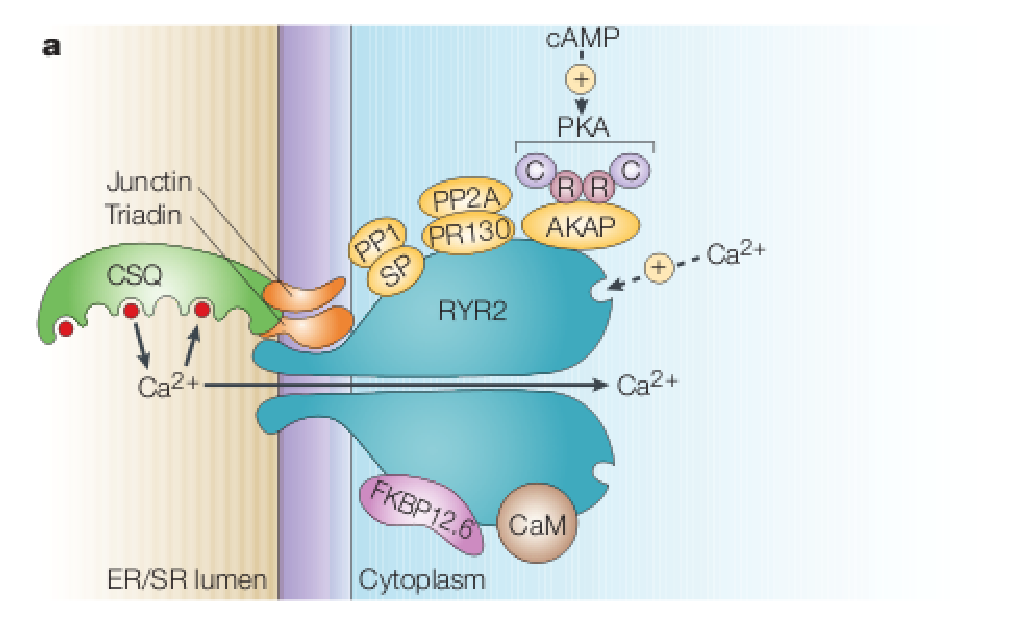
\includegraphics[height=8cm]{./images/RyR2.eps}}
  \caption{RyR2}\label{fig:RyR2}
\end{figure}

As cardiac myocyte is the target, we're focusing on RyR2 only. RyR2 is
composed of 4 subunits that form the channel, as shown in
Fig.~\ref{fig:RyR2}.  Inside the ER/SR, the Calsequestrin (CSQ) is a
low-affinity high-capacity \ce{Ca^2+}-binding proteins that helps
ER/SR stores an amazing amount of calcium. Its interaction with RyR2
is facilitated by the transmembrane protein {\it triadin} and
{\it junctin} in such a way that modulates the sensitivity of
RyR2\footnote{\url{http://www.med.uc.edu/kranias/calsequestrin.html}}. During
systole, CSQ coordinately releases $\approx$ 40-50\% \ce{Ca^2+} ions
per molecule for each contraction-relaxation cycle by an uncertain
mechanism.

The reversible phosphorylation of RyR2 by cyclic AMP
(cAMP)\footnote{cAMP is derived from ATP} is controlled by protein
kinase A (PKA), a cAMP-dependent protein kinase, which is composed by
a regulatory (R) and catalytic (C) subunits that are attached through
an A kinase anchoring protein (AKAP).  RyR2's dephosphorylation
depends on protein phosphatase 2A (PP2A), which is attached through
the isoleucine-zipper-binding scaffolding protein PR1130 and on
protein phosphatase (PP1), which is attached through spinophilin (SP).
RyR2 is also modulated by calmodulin (CaM) and FKBP12.6. Its 3D
structure is further described in detail at
\url{http://www.wadsworth.org/rvbc/ryano.htm}.

Even now, the understanding of RyR is still far from
completeness. Thus, it is important to understand how individual RyR
is regulated and, specifically, how CICR is controlled. There is the
agreement that the control of RyR function, at least pertain to CICR,
is a local property, i.e. \ce{Ca^2+} release in the CICR process is
heterogeneous at different release site (CaRU). However, there is
still disagreement about the underlying self-regulatory mechanism that
would cause RyR to terminate.

The activation of RyR is complex, especially the complex kinetic
behavior with multiple gating modes (e.g. 6-states or 12-states) and a
complex inactivation patterns that occur at a relative high
[\ce{Ca^2+}] ($>1\mu$M). The central issues is whether RyR can adapt
to the local [\ce{Ca^2+}] and how~\citep{gyorke1993ryr}. Here,
adaptation means that a local step [\ce{Ca^2+}] increase (to $<1\mu$M)
causes a {\it biphasic activation pattern} in single RyRs, i.e. a
rapid activation followed by a slow decrease in channel open
probability ($P_o$) and importantly, RyR can be reactivated by a
further local increase in [\ce{Ca^2+}].

\subsection{adaptation}
\label{sec:adaptation}

Other studies revealed that the \ce{Ca^2+}-dependent adaptation of RyR
channels, both activation and inactivation, is distinct from
conventional desensitization of membrane channels as these channels
cannot response to subsequent stimuli (due to inactivation
period). However,
\textcolor{blue}{RyR channels adapt to a maintained \ce{Ca^2+}
  stimulus and are thereby able to respond to subsequent \ce{Ca^2+}
  stimuli}, as shown in Fig.~\ref{fig:RyR_response}.  In particular,
the \ce{Ca^2+}-sensitive of RyR activation decrease during prolonged
exposure to \ce{Ca^2+}\citep{gyorke1993ryr}. This is due to the shift
in ligand sensitivity or it could be attributed to an interaction
between RyR and an unidentified regulatory protein
(inhibitor). Regardless of the mechanism, {\bf adaptation} is a
fundamental feature of intracellular \ce{Ca^2+} release channels,
particularly in RyRs.
\textcolor{red}{Adaptation is often characterized by a fast
  activation and a slower inactivation}.
Such single-channel adaptation may not be unique to RyR, e.g. the
incremental \ce{Ca^2+} release from IP3-sensitive \ce{Ca^2+} stores.



\section{Distribution}
\label{sec:RYR-distribution}

\subsection{In peripheral}
\label{sec:peripheral}

The peripheral RyR clusters, which occur in junctions between the
terminal SR and the surface membrane. Using the high resolution
imaging technique ($\sim 30$nm),~\citep{Baddeley2009} has provided
some insights into these clusters.

\subsection{In CRU}
\label{sec:cru}

RyRs are thought to cluster in a CRU in a ``quasi-crystalline'' arrays
with a unit cell size of $\sim$ 30 nm~\citep{Yin2000}.The narrow gap
between the SR and sarcolemma membrane is $\sim 10-15$ nm. 

Typically, the assumption of circulation and complete filling of the
junction by the close-packed RyR is utilized. However, the new imaging
result revealed that these key assumption may not be
correct~\citep{Baddeley2009}. In fact, RyR cluster have a complex
geometries.

Due to the site to site variability in number of RyRs, there should be
an autoregulation mechanism (e.g. luminal SR depletion, or luminal
gating). Otherwise, it may lead to a $>5$-fold variation in spark
amplitude, which is not physiological. 


The cluster size distribution can be explained by a stochastic process
of cluster growth~\citep{Baddeley2009}. 

\section{Regulatory factors}
\label{sec:ryr_regulation-factors}


The activation of the other two types (RyR2, RyR3) is governed by a process
known as calcium-induced calcium-release (CICR) where RyR(2,3) couples a local
increase of calcium influx from the opening of proximal DHPR channels on the
T-tubules. 

RyR is activated and/or inhibited by calcium, and is regulated by ryanodine,
FK506-binding proteins. RyR is regulated by ryanodine via allosteric coupling of
interaction with both high affinity ($\Kd\sim 10$nM), and low affinity ($\Kd\sim
1\mu$M) ryanodine-binding sites~\citep{Lai1988d,Wang1993}.

Other key regulators of RyR involve $\Ca$ (activate/inactivate), $\Mg$
(inactivate), caffeine (activate) and ATP, as well as accessory proteins
(triadin/junctin and transmembrane protein in jSR - CASQ
(Sect.\ref{sec:calsequestrin}), annexin (Sect.\ref{sec:annexin}), calmodulin
(CaM), FKBP12/12.6). There are also many more agonists and
antagonists~\citep{Dulhunty2007,Santonastasi2007}. A mechanistic model of RyR
kinetics should also take into account the affect of these proteins.

There are also other agents involving regulating RyRs that activate RyRs: agents
that modify sulfhydryl (SH) groups, e.g. SH reagents, free radicals, and
hydrogen peroxide, heavy metals, mercurials, dithiodipyridines, derivatives of
nitric oxide \citep{marengo1998}. SH reagents shift the calcium activation curve
to the left, while heavy metals enhance calcium sentivity of tension
development (see Sect.\ref{sec:redox_SHgroup}). 

In early days, $[\Ca]$ is the widely accepted agonist to RyR2. Nowadays, we have
learnt that RyR is not solely dependent upon $[\Ca]_i$. At resting $[\Ca]_i$
level, RyR open probability is not zero, though very small. RyR can be
phosphorylated \citep{valdivia1995, marx2000} which increase the opening
probability. Some studies suggested that ``hyperphosphorylation'' in heart
failure leads to a decrease in SR content \citep{marks2001}, yet some don't
agree \citep{bers2003}.

The level of calcium leak via RyR2 has been shown an important role to cardiac
failure. Thus, RyR2 is being considered as the novel target for thereupatic
drugs development. This requires a full and complete understanding of functional
role of RyR accessory proteins.

\subsection{Intrinsic features}

It's suggested that interaction between cytoplasmic and transmembrane domain of
the channel itself is an important mechanism in the intrinsic modulation of RyR
$\Ca$ release channels \citep{george2004}. Carboxyl-terminal portion (20\% of
the sequence) in the skeletal muscle is the part that determine the functional
form of RyR1 \citep{Bhat1997}. They also discovered that the high-affinity
calcium binding site in RyR1 reside in the C-terminal portion, but not the
low-affinity calcium binding site.
 
\subsection{Subspace-$\Ca$ dependent}
\label{sec:RyR_subspace_Calcium}

RyR1 in skeletal muscle has a biphasic $\ca$-dependent (a bell-shape cytosolic
$\Ca$-dependence curve), i.e. it activates the channel at low $[\ca]$ ($\mu M$)
and inactivates at higher $[\ca]$ (mM)~\citep{Bull1993,Percival1994} [NOTE:
Bull1993 has erratum in FEBS Lett 1994 Jan 3;337(1):121]. This is called {\it MS
calcium dependence} (MS=mammalian skeletal). The threshold for RyR1 channel
activation is about 4.5$\muM$ (Hill coefficient 1.46), and blocking constant is
226$\muM$ (Hill coefficient 1.42). The RyR1 channel is almost completely
inhibited at milimolar range of $\Ca$, i.e. no blocking effect was seen with
calcium $\ge 0.5$mM. So, it was hypothesized that RyR1 channel has a
high-affinity activating $\Ca$-binding site, and a low-affinity inactivating
$\Ca$-binding site.

Unlike RyR1 in skeletal muscle, RyR2s, as well as RyR3, are less susceptible to
inhibition of cytosolic $\Ca$. Data shown that at least 10x more $[\ca]_i$ is
required to inactivate the channels~\citep{Bhat1997}. So, in cardiac cell, it
displays a sigmoidal activation, Fig.\ref{fig:RyR_Po}. This is called C calcium
dependence (C=cardiac). That explains why \textcolor{red}{the inactivation O
$\rightarrow$ C of RyR2 for ventricular myocytes is often modeled as
$\Ca$-independent}.

\begin{figure}[hbt]
  \centerline{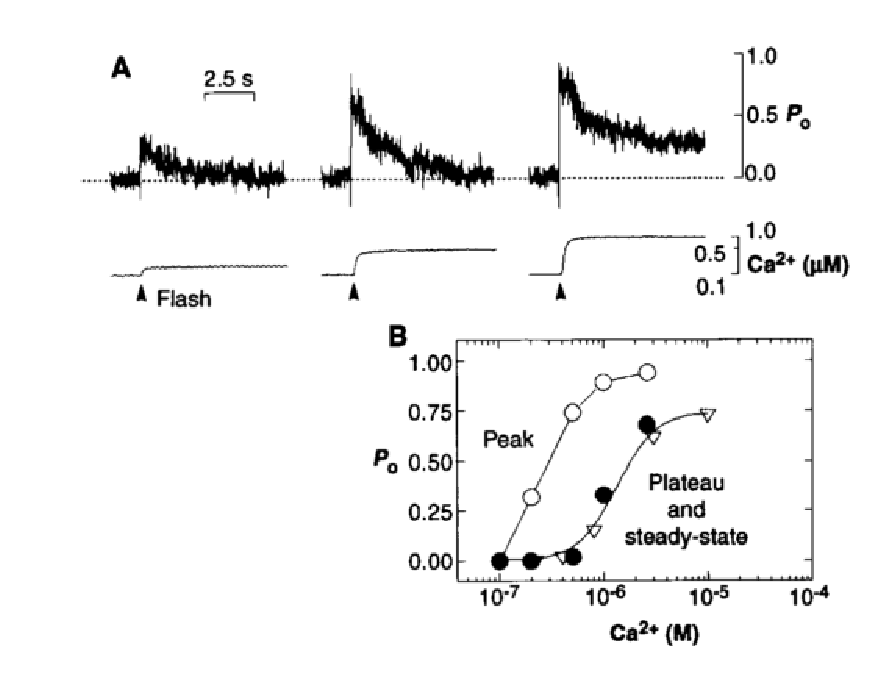
\includegraphics[height=7cm,
    angle=0]{./images/RyR_Po.eps}}
\caption{(A) Single channel P$_o$ measured, during sustained $\Ca$ stimulus with
$[\Ca]=$ 0.2, 0.5 and 1$\muM$ (level of calcium before the stimulus is
0.1$\muM$); (B) Calcium-dependence of P$_o$ (steady-state conditions is
measured at constant $[\Ca]$ over several minutes)\citep{gyorke1993ryr}}
\label{fig:RyR_Po}
\end{figure}


\begin{framed}
  Resting free cytosolic $[\ca]$ is near 100nM, while in the SR is
  about 1mM [....pg900]. In addition to $\ca$, the cytosol contains a
  complex mixture of salts ($\sim 140$ mM $\K$, $\sim 1$mM $\Mg$, 5-10
  mM ATP, and various other nucleotides) [...].
\end{framed}

In brain cortex neuron, RyR channels have displayed 3 types of responses: C and
MS calcium dependencies, and low P$_o$ calcium dependence \citep{marengo1996,
bull2007}. The third one, characterized by a bell-shaped calcium dependence with
fractional open time les than 0.1 in the calcium range 0.1$\muM$ to 0.5$\muM$,
is observed with the highest frequency. This third response is also found in
mammalian skeletal RyR channels \citep{copello1997}. In essence, only RyR
channels in the cardiac cells don't display the third properties,
Fig.\ref{fig:RyR_Po_mode}. 

\begin{figure}[hbt]
  \centerline{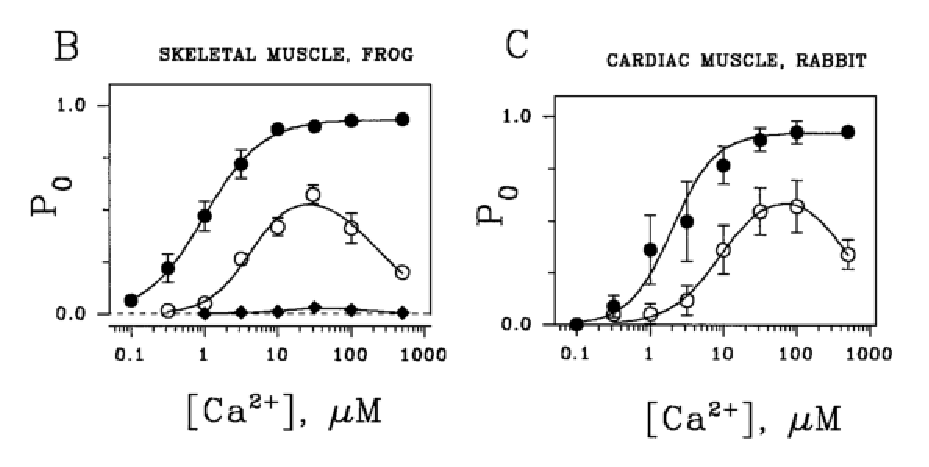
\includegraphics[height=5cm,
    angle=0]{./images/RyR_Po_modes.eps}}
\caption{(B) Skeletal channels display all 3 response: ($\blacklozenge$):
low $P_o$ calcium-dependence, ($\bullet$): C calcium-dependence, and ($\circ$):
MS calcium-dependence \citep{marengo1998}}
\label{fig:RyR_Po_mode}
\end{figure}

The curve in Fig.\ref{fig:RyR_Po_mode} is fitted with experimental data using
\begin{equation}
P_o = P_{o,\max} \times \frac{1}{1 + \left( K_a/[\Ca] \right)^{n_1} + \left(
[\Ca]/K_i \right)^{n_2} }
\end{equation} 
$P_{o,\max}$ is the theoretical $P_o$ value of maximum activation by calcium.
$K_a, K_i$ corresponds to calcium concentration at half-maximum activation and
inhibition of channel activity. $n_1,n_2$ is the Hill-coefficient for activation
and inhibition. See Table 1 in \citep{marengo1998} 
\begin{itemize}
  \item Low P$_o$ calcium-dependence: $n_1=n_2=1$
  \item MS calcium-dependence: $n_2=n_1$ with values depending on species
  \item C calcium-dependence: $K_i>5$mM, $n_2=0$, while $n_1$ with values
  depending on species
\end{itemize}

Mathematical that models the $\Ca$-dependent inactivation of RyR:
\citep{wang2004, rovetti2010sis} used the stochastic cardiac couplon 4-state
model of \citep{stern1999lcm} (Sect.\ref{sec:RYR_Stern1999}),
\citep{shannon2004} which extended the model of \citep{stern1999lcm} by adding
lumenal calcium dependent activation/inactivation
(Sect.\ref{sec:RyR_Shannon2004}), \citep{Lee2008} (Sect.\ref{sec:RyR_Lee2008}),
\citep{Liang2007} (Sect.\ref{sec:RyR_Liang2007_2009}), \citep{Krishna2010} ,
\citep{Hashambhoy2010} modified \citep{shannon2004} by estending into 8-state
with the new 4-states (phosphorylated) mirrored the old 4-state
(unphosphorylated) (Sect.\ref{sec:RyR_CaMKII_Hashambhoy}), \citep{laver2012}
(Sect.\ref{sec:RyR_Laver2012}), \citep{Cannell2013}.
Until recently, \citep{Liu2013} has pointed out that models that omit $\Ca$-depenent
inactivation produce more realistic results that those that continue to assume a
prominent role of RyR inactivation in cardiac myocytes. Models belong to this
group are: \citep{Gaur2011} (Sect.\ref{sec:RyR_Gaur2011}).
 
It was suggested that RyR activation requires the binding of 2-4 $\Ca$ ions
\citep{Sitsapesan1994, Zahradnik1999}.

\subsection{Luminal-$\Ca$ dependence}
\label{sec:RyR_luminal_Calcium}

Even though CSQ, triadin and junction were supposed to involve into
regulating RyR, the cellular mechanism for sensing changes in SR $\Ca$ is still
not clear \citep{Sobie2012}. Planar lipid bilayer showed that isolated RyRs have
lumenal $\Ca$ binding site \citep{laver2007}. With CSQ, the effect of lumenal
$[\Ca]_\jsr$ on RyR gating is much greater. However, \citep{qin2008}
hypothetized CSQ has activation role on RyR, while \citep{Gyorke2004} believed
it has inhibition role.

The rate of $\Ca$ release is inevitably dependent upon SR $\Ca$
content~\citep{Donoso1995,Lamb2001}. Even though increase in luminal calcium
increase augments channel activity by increasing the channel sensitivity to
agonists (cytosolic $\Ca$, ATP, and caffeine), if it passes a certain threshold,
it causes a decreases in channel activity. Lumincal $\Ca$ regulation can be an
intrinsic property or is created by an accessory protein. There are evidence to
support both hypothesis:
\begin{itemize}
  \item an activating and inactivating luminal $\Ca$-binding
sites~\citep{ching2000}. It's suggested that there's a $\Ca$-sensing site on the
luminal side of the RyR complex.

  \item the dissocation of calsequestrin (CSQ), triadin and junctin abolished
  RyR2 regulation by luminal $\Ca$~\citep{Gyorke2004}, and CSQ association
  amplified channel responses to luminal $\Ca$~\citep{Beard2005}.
\end{itemize}

Partial depletion of $[\Ca]_\jsr$  is considered a key factor in spark
termination \citep{7,11-13}. However, the question is the critical threshold
of $[\Ca]_\jsr$ for spark termination, if it plays a role? 
\begin{enumerate}
  \item \citep{zima2008tcas} estimated the threshold for spark termination is SR
  $\Ca$ reach $\approx 60\%$ of resting $[\Ca]_\jsr$, independent of SR $\Ca$
  load or release flux. Despite this constant of $[\Ca]_\jsr$ nadir, there is a
  wide variation in blink recovery time among CRUs.
\end{enumerate}


\subsection{$\Mg$ dependence}
\label{sec:RyR_Mg_inactivate}

$\Mg$ is a potent RyR channel inhibitor. At milimolar range, $\Mg$ inhibit RyR
completely~\citep{}, which is a significant mechanism to keep RyR1 close. RyR2
and RyR3 is sensitive to $\Mg$ to a lesser extent.


\subsection{ATP dependence}
\label{sec:RyR_ATP_dependence}

ATP, at milimolar range, is a potent agonist of skeletal muscle RyR

\subsection{Dephosphorylation}
\label{sec:RyR-dephosphorylation}


Dephosphorylation is carried out primarily by protein phosphatase 1 (PP1), and
protein phosphatase 2A (PP2A - Sect.\ref{sec:PP2A}).

\textcolor{red}{RyR association with CaMKII is direct; while RyR association
with PKA, PP1 and PP2A is indirect}, i.e. through specific anchoring proteins.

\subsection{Phosphorylation}
\label{sec:RyR_phosphorylation}

RyR2 contains 3 leucine-isoleucine zipper (LIZ) motifs:
\begin{itemize}
  \item one mediate PP2A binding (possibly through B'' regulatory subunit PR130)
  \item AKAP6 (mAKAP - Sect.\ref{sec:AKAP}) binds to the second LIZ
  \item spinophilin bind to the third LIZ
\end{itemize}

RyR1 in skeletal muscle lacks LIZ motif that mediate PP2A binding, thus only
work with PP1 and PKA.

Both RyR1 and RyR2 are substrates for phosphorylation by serine/theronine
protein kinases (Sect.\ref{sec:serine-thereonine_protein-kinases}) in which the
two major protein kinases are cAMP-dependent protein kinase A (PKA -
Sect.\ref{sec:PKA-RyR}) and $\Ca$-calmodulin-dependent protein kinase II (CaMKII -
Sect.\ref{sec:CaMKII}), and a less efficiently contribution from cGMP-dependent
protein kinases (Sect.\ref{sec:cGMP}).

Functional effect of RyR phosphorylation and dephosphorylation have been studied
by SR $\Ca$ flux measurements, single channel recording and by ryanodine-binding
assays, which show
\begin{enumerate}
  \item $\beta$-adrenergic stimulation leads to cAMP elevation and PKA
  activation, resulting in enhancement of EC-coupling. This is due to: increased
  DHPR $\Ca$ current, higher SR $\Ca$ content cuased by higher SERCA pump
  activity following relief phospholamban inhibition. 

  \item The effect of $\beta$-adrenergic stimulation on RyR has been found to
  up-regulated, despite lower SR $\Ca$ content~\citep{Lindegger2005}. Even
  though, it did enhance initial SR $\Ca$ release, PKA-mediated phosphorylation
  (and $\beta$-adrenergic stimulation) was found no effect on
  EC-coupling and $\Ca$ transient~\citep{Ginsburg2004}.
 
 \item The effect of PP1 and PP2A in cardiac cells are unclear at present
 (2011), some reported decrease $\Ca$ transient and EC-coupling without
 affecting SR $\Ca$ content; and some otherwise.
\end{enumerate}

\subsection{-- PKA}
\label{sec:PKA-RyR}

PKA is discussed in Sect.\ref{sec:PKA}. 
PKA-mediated phosphorylation sites at RyR:
\begin{enumerate}
  \item  Ser2809
  
  \item Ser2030 
\end{enumerate}

Addition of exogenous PKA:

  \begin{itemize}
    \item increase RyR activity (due to enhance   sensitivity of $\Ca$
    activation and substantially reduce $\Mg$ inhibition).  This effect is reversed by PP
    
    \item PKA activated RyR only occur during rapid rises in local $\Ca$
  concentration; and promote channel closure under fixed $\Ca$ level.
  
    \item PKA-stimulatory effect only occur when stoichiometric phosphorylation
  of S2808 is achieved; thus phosphorylation by up to 75\% (as in normal heart at
  rest) has no effect on channel activity.
  \end{itemize} 

Example: AKAP6-anchored PKA increase $P_o$ of RyR2.
This explains why computational model take into account the effect of CaMKII
first~\citep{greenstein2002}. Evidence suggested there are many sites on RyR
phosphorylated by CaMKII.
  

The discovery of Marks {\it et al.} that hyperphosphorylation of RyR
could underlie abonormal calcium cycling in heart failure has raised
many debate~\citep{marx2000}. It was found that PKA phosphorylation
regulates the binding of FKBP12.6 to the RyR by dissociating FKBP12.6
from RyR~\citep{Takasago1991}. So,
\textcolor{red}{PKA phosphorylation is often found in failing hearts},
increasing from about 1 site out of 4 was phosphorylated in normal
heart to 3 sites phosphorylated in failing heart~\citep{marx2000}. To
avoid heart failure, PKA inhibitor PKI$_{5-24}$ (500nM) can be
used. The stoichiometry of PKA phosphorylation is $3.8\pm 0.1$ moles
phosphates per mole of channel, suggesting that, with four subunits,
each phosphate goes to one subunit or PKA phosphorylation occurs at a
single amino acid residue.

\subsection{-- CaMKII}
\label{sec:CaMKII-RyR-phosphorylation}

Not only PKA, but also CaCalmodulin-activated kinase II (CaMKII) also
phosphorylate RyR~\citep{Wehrens2004b}. 

Addition of exognenous CaMKII:
\begin{itemize}
  \item enhance RyR channel activity
  \item one report decrease activity~\citep{}
\end{itemize} 



\subsection{KF506-binding protein (FKBP12.6 for RyR2; FKBP12 for RyR1)}
\label{sec:RyR_FKBP}
\label{sec:FKBP}

FKBP12.6 is  the 12.6 kDa protein binding to the immunosuppressive drug FK506;
aka Calstanbin2~\citep{wehrens2003}. FKBP12 is  the 12 kDa protein binding to
the immunosuppressive drug FK506.

Each subunit of RyR2 binds with FKBP12.6 ~\citep{marx2000}; while the accessory
proteins for RyR1 is FKBP12. Both FKBP12 and FKBP12.6 are inhibited by FK506 and
rapamycin, in a concentration-dependent manner.
Although both FKBP12 and FKBP12.6 are expressed in the heart, and FKBP12 is
considerably more abundant than FKBP12.6, only FKBP12.6 co-immunoprecipitated
with RyR2.

FKBP12.6 are regulatory units that stabilize RyR channel functions (RyR1 in
skeletal muscle~\citep{brillantes1994}, RyR2 in cardiac
cells~\citep{Kaftan1996}, IP3R1~\citep{Cameron1997} and type I TGF$\beta$
receptor (T$\beta$RI)~\citep{Chen1997}) and facilitates coupled-gating between
neighboring RyR2~\citep{marx1998}.


Both types share 85\% in homology. The structure, determined by X-ray
crystallography, were almost identical, and unaltered in their drug complexes.

\begin{framed}
  FK506, known as tacrolimus (or fujimycin), is an immunosuppressive
  drug used in allogeneic organ transplantation to reduce the risk of
  organ rejectioin.  FK506-binding proteins for RyR1 is FKBP12 (or
  calstabin1). The FK506-binding proteins for RyR2 is FKBP12.6 (or
  calstabin2). FKBP12.6 has 85\% homology with KFBP12. The
  stoichiometry of binding to RyR is 1 FKBP to 1 RyR monomer. 

  The removal of FKBP from RyR can be done by increasing KFBP506 level
  or its analogue, FK590. 
\end{framed}

FKBP12 serves to stabilize the closing state of RyR channels. The stoichiometry
of binding is 1 FKBP12 to 1 RyR subunit. RyR1-FKBP12 binding when the channel is
in its open state ($\Kd \sim 1$ nM) is quite strong, and is enhanced 4-5 folds
when the channel is in closed state. In canine, RyR2 bind to FKBP12.6
exclusively. In other mammalian verteberates (chicken, fish, frog), RyR2 can
also bind to FKBP12, though with 7-8 fold lower affinity. In some species, RyR2
is capable of binding both FKPB12/FKBP12.6 with the same affinity.

FKBP12 help stabilizing RyR, i.e. RyR reach full conductance level
($> 400\%$), decreasing opening probability $P_\circ$ after caffeine
activation (from $0.63\pm 0.09$ to $0.04\pm 0.02$), and increase
mean open time (from $4.4\pm 0.6$ms to $75\pm 41$ms).  FK506 or
rapamycin, inhibitor of FKBP12 in a concentration-dependent manner,
can reverse these stabilizing effects~\citep{brillantes1994}.

Dissociating of FKBP12.6 from the subunit may significantly alter the
biophysical properties of the channels, leading to a
{\bf subconductance state} or ``leaky'' RyR, and increase $P_\circ$
(about 3 times) due to an increase in $\ca$-sensitivity to
$\ca$-activation~\citep{Kaftan1996}, i.e. shifting the $\ca$
dependence for activation to the left.  Another effect that
dissociating may trigger is the inhibition coupled-gating,
i.e. individual channels gate stochastically rather than in an
ensemble~\citep{marx1998}.

\begin{framed}
Three residues on FKBP: Q31, N32, and F59 are critical for selective binding of
FKBP12.6 to RyR2. The involement of enzymatic isomerase is not required for the
binding. However, the binding sites on RyR is still controlversy. A unifying
hypothesis is that the binding site is formed by interacting domains, and is
disrupted when the inter-domain interactions is  disrupted.
\end{framed}

Functional effects of FKBP12 on RyR have been studied by using FK506 or
rapamycin to dissociate FKBP12, which results into an enhancement in channel
activity or the condition leading to the so-called ``leaky'' channels.
This is the result of increasing channel sensitivity to $\Ca$ and caffeine
activation and reduced sentisity to milimolar $\Ca$ and $\Mg$ inactivation. It
was also found FKBP12-deficient RyR open at a subconductance level
(approximately 25\%, 50\% and 75\% of the maximum conductance); though not
always be recorded.  Besides, FKBP12/12.6 binding have found to increase
functional coupling between adjacent RyRs in the array (``coupled gating'') to
promote channel closure. 

\begin{framed}
  Neither $\ca$ Calmodulin Kinase (CaMKII) nor protein kinase C (PKC)
  dissociate FKBP12.6 from RyR2. Hyperphosphorylation destabilize the
  association of FKBP12.6 or calstabin-2 to RyR2 channel. Fixing a
  leaky calcium channel could be a promising approach for protecting
  against life-threatening cardiac arrhythmias. Drugs like JTV519 can
  help stabilizing, by enhancing binding of calstabin-2 to
  RyR2~\citep{Wehrens2004}.
\end{framed}

It's hypothesized that through the action of PKA whose level is increased under
chronic hyperadrenergic state during HF, cause ryanodine receptors to become
hyperphosphorylated \citep{marx2000, marks2002}. This leads to a persistent
dissociation of KFBP from RyR, causing RyR to open more often, leading to low SR
$\Ca$ content \citep{marx2000, ono2000, yano2003, wehrens2003}. The low SR $\Ca$
content can lead to reduced contractility of the heart muscle, a condition
leading to congestive heart failure (CHF). A detail discusson will be coverred
in Sect.\ref{sec:heart-failure-hf}. The mathematical analysis of this effect is
discussed in Sect.\ref{sec:allosteric-coupling}.


\subsection{Ryanodine}

In cardiac muscle, ryanodine promotes $\ca$ leaks from intracellular stores
because it \textcolor{red}{ locks the RyR channels in the long-lived
  subconduction state} (with mean open time $\tau_o = 2.1\pm 0.8$ms in full
  conductance level to $\tau_o=502.1\pm 40.8$ms in subconduction
  state)~\citep{marx2000}. This ``leaked'' $\ca$ is rapidly removed from the
  cell by the relatively strong surface membrane extrusion mechanism
  (NCX)~\citep{Bers1990}.
In contrast, skeletal muscle lacks this strong surface membrane extrusion
mechanism, i.e. ryanodine-induced $\ca$ leak from SR cause $\ca$ to accumulate
in the cytoplasm and resulting in abnormally high cytoplasmic $[\ca]$ levels.

The C-terminal of RyR is the site for ryanodine binding \citep{callaway1994,
witcher1994}. 


{\bf Ruthenium red} is Ruthenium containing red staining dye. It can
bind to RyR and inhibit the release of $\Ca$ at nanomolar
concentration ($K_d=20$nM). It also inhibits $\Ca$ uptake by isolated
mitochondria.

\subsection{Calmodulin (CaM)}
\label{sec:RyR_CaM}
\label{sec:RyR-Ca2+-calmodulin}

Sect.\ref{sec:calmodulin} describes in details. CaM bind all three RyR isoforms
at nanomolar affinity irrespective RyR is Ca-free or Ca-bound. The stoichiometry
is one CaM bind to one RyR subunit.

\begin{verbatim}
Michel Puceat - Calmodulin: a gatekeeper for RyR function 
in the myocardium, Cardiovascular Res. 2010, 87
\end{verbatim}

In RyR1: CaM has a biphasic, $\Ca$-dependent effect on RyR1 activity which
activate the channel at low $\Ca$, and inhibit the channel at high $\Ca$ ($\ge 1\mu$M).
However, \textcolor{red}{CaM is not essential for EC-coupling}. In skeletal
muscle, CaM was shown to increase $\Ca$ spark frequency, whereas other spark
proeprties was unaffected. It thus suggests a role of CaM in activation, not in
termination $\Ca$ release~\citep{Rodney2003}. 

In RyR2: CaM inhibit RyR2 at all level of $\Ca$ concentration; although the
inhibition is more pronounced at high level of [$\Ca$]. Thus, some sugggested
CaM can serve to terminate SR $\Ca$ release. However, the time scale for
association and dissociation from RyR2 is very large (seconds to
minutes)~\citep{Balshaw2001}. So, a better hypothesis is that CaM play a
facilitatory role in $\Ca$ release termination, but not critical~\citep{Xu2004}


\subsection{Sorcin}
\label{sec:RyR_sorcin}
\label{sec:sorcin}

Sorcin interacts not only with RyRs (to inhibit RyR), but also with other
proteins involving in Ca-regulation like Na-Ca
exchanger~\cite{Rueda2006,Zamparelli2010}. Sorcin decreases the amplitude of
$[\Ca]_{ds}$ elevation, but not the amplitude of $I_\ca$. So, Sorcin reduce the
``gain'' of EC-coupling~\citep{Farrell2004}. Even though Sorcin has been shown
to inhibit calcium sparks, and to reduce moderately the amplitude of whole-cell
calcium transient; there is however no direct data supporting that Sorcin plays
a role in physiological process (Sect.~\ref{sec:RyR_sorcin}).



\subsection{Calsequestrin, Triadin, and Junctin}
\label{sec:RyR_CSQ_Triadin_Junctin}

Calsequestrin (CSQ) is found mostly in the jSR, not in the network SR
\citep{Jorgensen1984}. Calsequestrin (CSQ) is the most abundant calcium-binding
protein residing in the SR lumen \citep{ikemoto1972, beard2004}.
There are two genes encoding calsequestrin (CSQ): CSQ1 and CSQ2. CSQ1 is found
mainly in skeletal muscles, and CSQ2 is found mainly in cardiac cells.

CSQ is anchored to the junctional face SR membrane through the interactions with
two SR integral proteins; triadin and junctin. These four proteins (RyR2, CSQ,
triadin, junctin) form a quarternary ``RyR complex'' \citep{zhang1997},
Fig.\ref{fig:RyR_scheme_Lee2008}. Here, triadin and junctin are
anchoring proteins between CSQ and RyR. However, there is evidence that CSQ-1
can bind directly to RyR, at least in {\it C. elegans} \citep{Cho2007}.

\citep{MacLennan1971} estimated CSQ with a concentration of 10-20mM.
\citep{shannon1997} estimated that the total of $\Ca$-binding CSQ sites is about
15mM, which is closed to the estimated maximum calcium bound to buffer in the SR
14mM. Overexpression of CSQ delays SR amplitude restitution while
underexpression expedites the SR amplitude restitution \citep{terentyev2003cdf}.
Furthermore, mutation in CSQ have been linked to a cardiac disorder known as
CPVT (catecholamine-induced polymorphic ventricular tachycardia). For patients
with CPVT, exercise or stress can lead to fibrillation and sudden death
\citep{Lahat2001}.

At low $[\Ca]$, CSQ can associate with RyR complex, and inhibit RyR openings
\citep{ikemoto1989prc}. At high $[\Ca]$, when $\Ca$ ions bind to CSQ, $\Ca$
binding causes a conformational change in CSQ, which prohibits CSQ from
interaction with the associated proteins in the RyR complex \citep{mitchell1988,
Gyorke2004, Gyorke2004a}. However, other evidences suggested that CSQ only
dissociate from RyR under either low calcium concentration ($< 10\mu$M) or very
high (10mM). Recent evidences suggest CSQ is dissociated from RyR at $[\Ca]_\jsr
\ge 4$ mM, and remains intact with RyR when $[\Ca]_\jsr$ in the range 1-3 mM
~\citep{Beard2005}. \textcolor{red}{NOTE:
Some models assume RYR opens under CSQ-dissociation under physiological calcium
concentration (1mM). This may not be correct due to the above fact}.

In essence, it's believed that CSQ serves as calcium buffers, which bind 50-90\%
of calcium (at rest with $>90\%$ are bound, giving only 1mM calcium free in the
jSR) \citep{ikemoto1989prc}. CSQ is a low affinity to calcium (with half-maximal
calcium concentration for calcium-binding $K_d = 400-600\muM$ under conditions
100-150 mM KCl, pH=7.0-7.5) \citep{mitchell1988, slupsky1987}, yet high capacity
$\Ca$-binding protein (20-50 calcium binding sites per molecule, i.e. average 40
mol $\Ca$ per one mol protein) \citep{MacLennan1971}. The $\Ca$ affinity of CSQ
is known to increase sharply with decreasing KCl. In vitro, the monomeric form
of CSA can absorb $\approx 15$ $\Ca$ ions; while the dimeric forms of CSQ can
absorb $\approx 60$ $\Ca$ ions per dimer \citep{park2004}. \citep{Donoso1995}
estimated $B_\jsr$ from 132-182 nmol of calcium/mg protein with $K_d = 1.21$ and
1.14mM in frog and rabbit skeletal muscle, respectively.
% \sout{$K_d=63\muM$} \begin{enumerate} \item $K_d = 0.5$ mM with $\approx 40$
% $\Ca$-binding sites per molecule \citep{mitchell1988, slupsky1987}
% \end{enumerate}


In a ingeneous experiment by \citep{Gyoerke2004}, they suggested that the
complex formed by CSQ, triadin and junctin1 work in concert to regulate RyR2.
Also, $\Ca$ doesn't seem to bind directly to RyR2, but via CSQ. In a purified
RyR2 has no change in $P_o$ when $[\Ca]$ is added, i.e. no direct binding.
However, the open probability reduces when triadin-1 and junctin (T/J) is added
after that; and further reduce when CSQ is added in the end. . CSQ1 seems to
reduces the activity of RyR1; while CSQ2 increases the $P_o$ of RyR2
\citep{wei2009uis}. 

The association of CSQ to RyR, though inhibit RyR opening probability, it
amplifies CSQ response to changes in lumenal calcium concentration. Also,
phosphorylation doesn't change the inhibition of CSQ to native RyR, in the
present of triadin and junctin \citep{Beard2005}.
At high lumenal calcium, CSQ bind to $\Ca$ and then reduce the inhibition effect
of CSQ on RyR opening. In other words, at high lumenal calcium, RyR tends to
open more often.

Upon $\Ca$ binding, CSQs form dimers, tetramers, and eventually polymers as
$\Ca$ concentration increases~\citep{wang1998}. Thus, it is thought to play a
far more important role than simply calcium buffers, e.g. regulating calcium
release in which CSQ couples with RyR through anchoring protein, e.g. junctin
and triadin \citep{Gyorke2004a, zhang1997}. {\it In vitro}, CSQN monomers
quickly form oligomers, e.g. forming dimers when $[\Ca]_\jsr > 500\muM$ {\it in
vitro} \citep{park2004}. Also, different polymeric forms of CSQ have different
buffering capacity. 


\begin{framed}
There are two isoforms of CSQ, comprising of 390 residues with 86\% homology.
Triadin is a 95-kDa membrane glycoprotein from junctional SR.
Junctin is a 26-kDa protein. Though both aims to dock CSQ, their individual
roles remain to be investigated further. 
\end{framed}

\subsection{Redox modifies calcium-dependence}
\label{sec:redox_SHgroup}

Redox-active molecules (Sect.\ref{sec:redox_reaction_ROS}) can significantly
increases in the heart under certain pathological condition (e.g.
ischemia-reperfusion injury), or the activation of some signal transduction
pathways. These changes can affect gating properties of different ion channels
(LCC, SERCA, etc.), including RyRs \citep{zima2006}.
Redox modulation of RyR activity is regulated by the modification of the {\it
sulfhydryl group} of cystine residues. These agents can (1) oxidize SH groups,
(2) reduce SH groups, or (3) S-nitrosylate SH groups. 




Oxidation of SH residues modifies calcium dependence of all single RyR channels,
regardless of the origin. Oxidation state of the channel is thus a decisive
factor in determining calcium dependence \citep{marengo1998}. 



\section{Single channel current (permeability)}
\label{sec:i_1ryr}

As RyRs are inside the cell, ion conduction through it cannot be measured using
standard whole-cell recording techniques. Single channel recordings are used
by incorporating RyR channels into a planar lipid bilayer.

\subsection{Conductance}

The RyR from skeletal muscle is large conductance pore that permate multiple
ions (both monovalent and divalent cations). Unlike sarcolemma membrane
channels, selectivity of RyRs are quite low. Even though $\Ca$ activates RyR,
RyR channel is a poorly selective $\Ca$ channel with very high conductance
(\sout{$\sim$ 700 pS} $\sim 400$pS when monovalent ions like $\K, \Cs$ are the
charge carrier, and $\sim 100$pS when $\Ca$ is the charger carrier)
\citep{Lai1988d, brillantes1994}. With $\Ca$ as the charge carrier, the maximum
conductance measured was 80 pS for RyR2, and 172 pS for RyR1
\citep{smith1988prr, lindsay1991, zucchi1997}. The conductance for monovalent
ions is higher, with 0.6 nS and 1 nS for the case of $\Na$ and $\K$,
respectively. Some studies showed that conductance for $\Ca$ with 135-150 pS,
and 7-fold faster for $\K$.

The explanation is that due to its localization, high-conduction pore is more
important than ion discriminization. RyR has a rather wide pore as it can
peremate relatively large molecule ($\Cl$, xylose whose radiuses are 2.9$\AA$
and 3.4$\AA$ respectively). This suggests a minimum width of RyR pore is
3.4$\AA$. The total lengh of the pore is about 10$\AA$ which is shorter than SR
membrane of about 45-50$\AA$. However, at normal condition, the gradient of $\K$
across the SR is almost zero, so most computational models for RyR only consider
the role of $\Ca$.

\begin{framed}
BLOCKING: Large organic and inorganic cations, anaesthetics and peptides were
shown to block RyR1 and RyR2 channel from
cytosolic side~\citep{Tinker1992, Tinker1992a,
Tinker1992b, Tinker1993}.

Polycations (neomycin~\citep{Mead2004}, ruthenium red~\citep{Xu1999}) can block
channels from both sides.
\end{framed}

RyR open at full conductance without ryanodine binding. RyR also exhibits
partially conducting states at submicromolar to micromolar ryanodine (up to
10$\mu$M). With one ryanodine binding at the high-affinity site, it locks the
channel at subconductance state, and inhibit ryanodine bindings to other
low-affinity sites in the tetramer. Experimental data suggested a single
high-affinity ryanodine-binding site per tetramer RyR channel, and 4
low-affinity ryanodine-binding sites, each on a subunit of the tetramer.

At high concentration of ryanodine, ryanodine can bind to the low-affinity
sites.  Occupation of these low-binding sites slow the dissociation of ryandoine
from the high affinity site, and then cause the channel to slowly transite to a
state characterized by persistent channel inactivation. This has been proposed
as the effect of allosteric and steric negative interaction between 4 identical
binding sites.   

\begin{framed}
The high-affinity binding site is found to localize at the C-terminal domain of
the protein. It has been also suggested that binding site reside at the channel
pore (M9 and M10 domains), as mutations at this regions affect the ability of
the receptor to bind ryanodine without affecting other characteristic of the
channel. Also, the interaction between ryanodine with RyR is voltage-dependent,
it suggests the binding site must be within the voltage drop across the channel
pore.
\end{framed}

Even though there are evidences of multiple subconductance states, the most
frequently observed one is the long lasting substate of 40-50\% of the full
conductance state. At higher level of ryanodine ($> 10\mu$M), the channel is
blocked.  At very low dose of ryanodine (10nM), the frequency of RyR openings
increase and lead the channel to full conductance level. For each RyR1 tetramer,
subconductances exist. 4 subconductance states were found, following the
dissociation of small accessory protein FK506-binding protein 12 (FKBP12). In
RyR2, the accessory protein is FKBP12.6.
At first, this lead to the hypothesis that each subunit has its own conduction
pore. However, \textcolor{red}{subconductance states can also be achieved in a
single pore (single ion-conduction pathway) and this model is consistent with 3D
structure of RyR} (Sect.\ref{sec:RyR_3D}).


\subsection{Single channel current}

Based on the conductance described above, single RyR channel current is from
0.07 - 0.35 pA \citep{mejia-alvarez1999, Kettlun2003, Guatimosim2002}.
Typically, the effect of luminal calcium depeletion is the phenomenon that is
expected to reduce the effective unitary current of RyR in vivo. So, in some
simulations that this effect is egnored, rather than using unitary current, they
may use effective current, which is now a small (non-realistic) ionic current,
e.g. 0.04pA\citep{groff2008}.

In 1999, with lumenal $\Ca$ less than 2mM, \citep{mejia-alvarez1999} measured
the unitary $\Ca$ current under physiological conditions should be $< 6$ (pA),
e.g. 0.35pA  when $[\Cs]=150$ (mM) symmetrical and no $\Mg$ at 0mV holding
potential, and saturating at 0.4pA.
To minimize gating fluctuations, \citep{Kettlun2003} used caffeine to measure
the $i_\ryr$ single RyR channel current (from lumen to cytosol) at 0 mV, which
gave 4.0-4.07 (pA) with 20mM lumenal $\Ca$. In physiological $[\Mg], [\K]$, and
lumenal $[\Ca]=1$ (mM), the single RyR current is $< 5$ (pA)\citep{Kettlun2003}.
Unitary RyR channel current $i_\ryr$ under physiological conditions
should be $< 0.6$pA and as low as 0.07pA in the presence of
physiological concentrations of $\Mg$. 

% \subsection{Subconductance states}
% \label{sec:RyR_conductance}


% , with $\sim 100$pS for $\ca$ and $\sim$400 pS for monovalent
% (\ce{K+},\ce{Cs+})
\subsection{Dwell-times}





%%% Local Variables: 
%%% mode: latex
%%% TeX-master: "thermo-stat"
%%% End: 
